\subsection{WBS}

\begin{figure}[H]
 \centering
  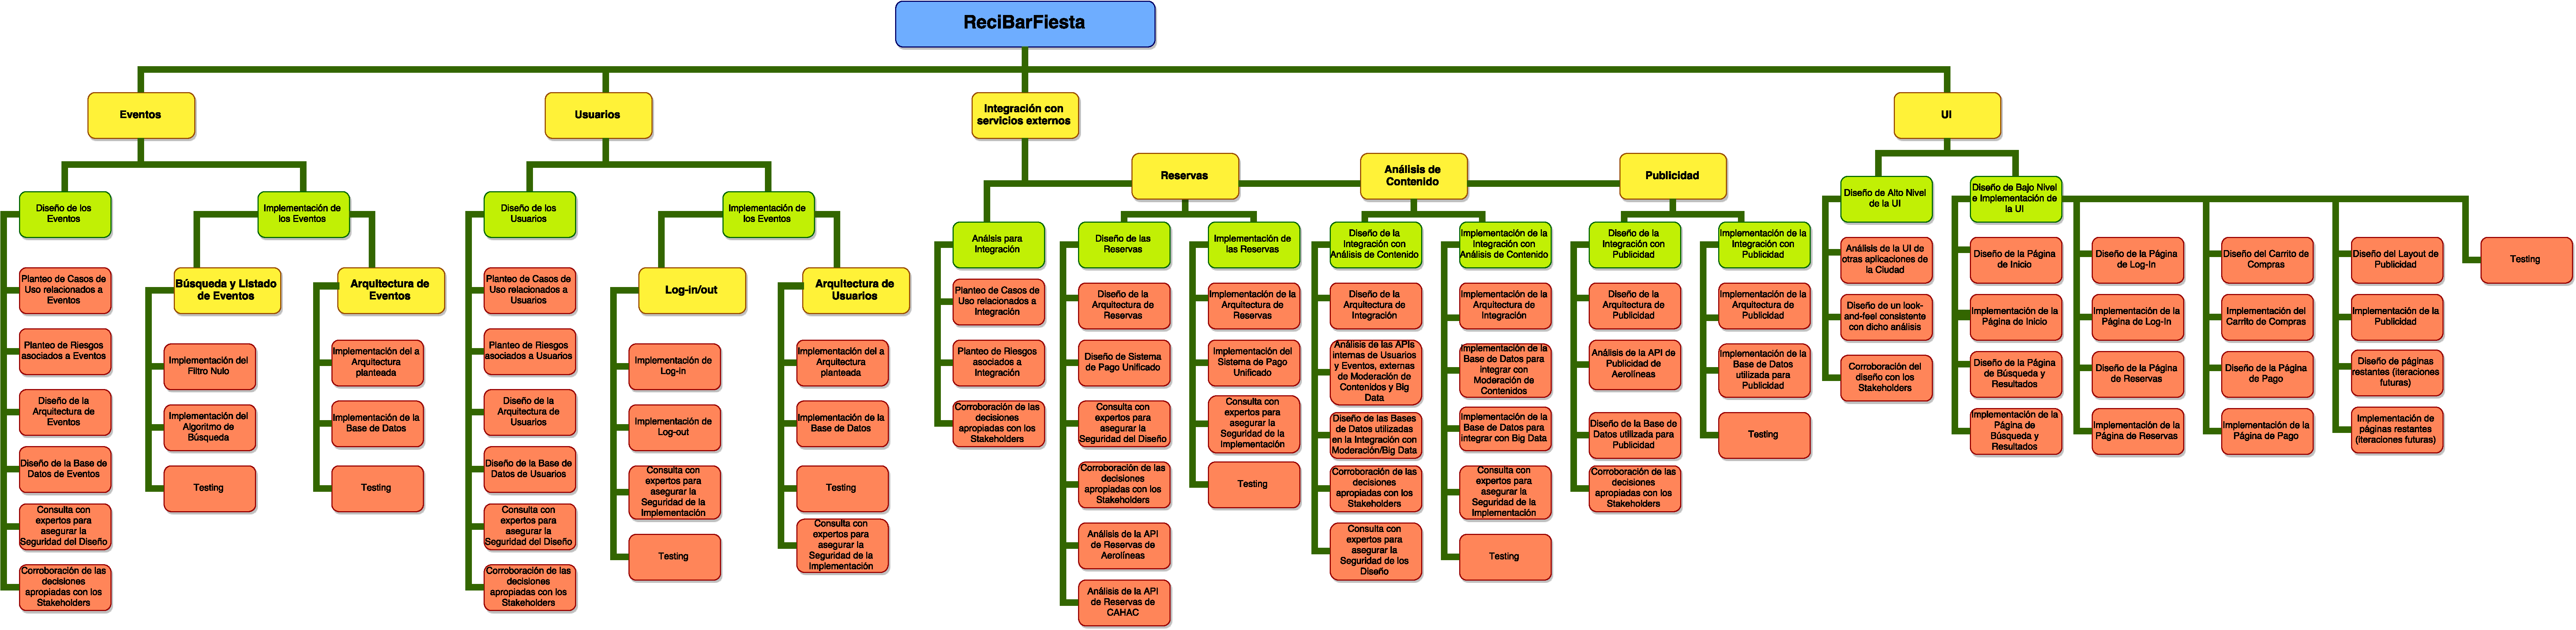
\includegraphics[width=\textwidth]{diagramas/WBS.pdf}
  \caption{WBS}
  \label{fig:wbs}
\end{figure}

En la figura \ref{fig:wbs} puede observarse el diagrama del WBS. Los nodos amarillos representan productos; los verdes, procesos; los rojos, tareas, independientemente de que sean productos o procesos.
Cabe realizar algunas aclaraciones respecto del diagrama. El diseño de la arquitectura del sistema se realizará para la próxima entrega; algunas de las subdivisiones en tareas se basan en dicho diseño, por lo que se observan múltiples instancias de tareas placeholder de la forma “Implementación de la Arquitectura de X”. Tras realizar dicha arquitectura, éstas se deberían separar en las tareas más granulares a realizar.
Es decir, en el WBS nos limitamos a presentar una visión de alto nivel de las subdivisiones del proyecto, que serían refinadas al proceder con el proceso de diseño. El enfoque más específico se reserva para los productos, procesos y tareas correspondientes a los Casos de Uso que fueron designados a la primera iteración.

\subsection{Primera iteración}
Para reflejar el orden en que llevaremos a cabo la primera iteración realizamos un diagrama de Gantt (figura \ref{fig:gantt}) el cual modela, entre otras cosas, las dependencias, duraciones y fechas de inicio de cada tarea; sirviendonos de guía al llevar a cabo el proyecto y para identificar puntos delicados en nuestro plan, utilizando criterios como el de camino crítico. 

\begin{figure}[H]
 \centering
  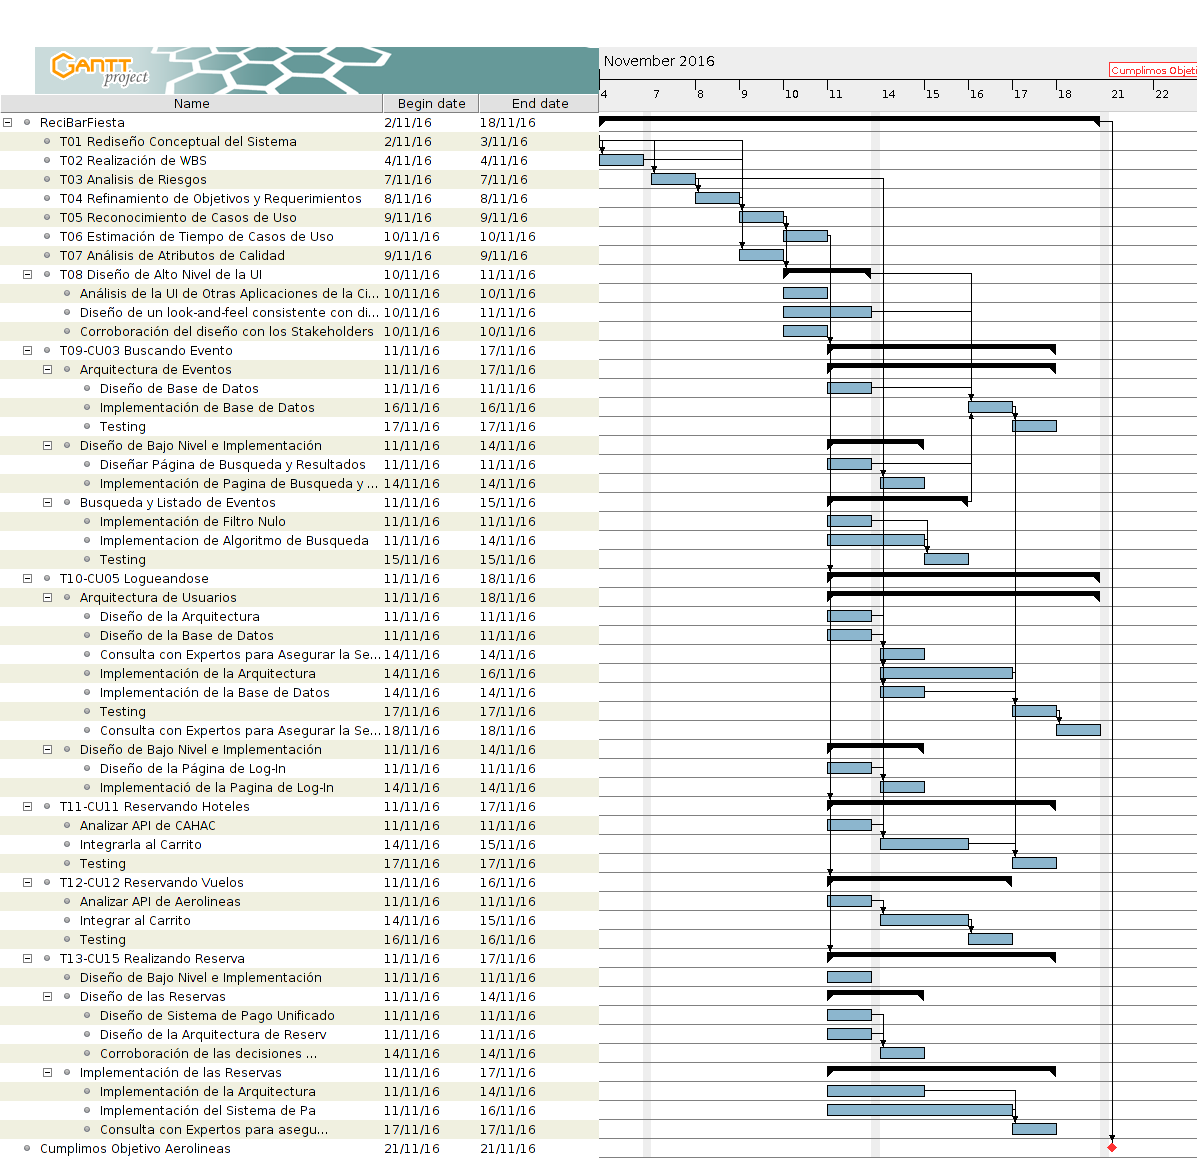
\includegraphics[width=\textwidth]{diagramas/gantt.png}
  \caption{Diagrama de Gantt para la primer iteración del proyecto}
  \label{fig:gantt}
\end{figure}

\subsubsection{Justificación}
Como vimos antes, deberíamos priorizar tener la integración con Aerolíneas Argentinas terminada lo más rápido posible, de tal manera de mitigar el riesgo de no tenerla terminada para 2017. Nótese que es el único riesgo que encontramos al cual tenemos exposición alta. De esta manera, pusimos en la primera iteración todo lo relacionado con la compra de pasajes de avión y reserva de hoteles. Esta es la parte más delicada de la integración. El cumplimiento de este objetivo se puede ver reflejado como un hito en nuestro diagrama de Gantt

Además, incluimos los otros dos casos de uso a la iteración porque son fundamentales para toda la aplicación en general, y para la integración con Aerolíneas en particular.

\subsection{Resto de las iteraciones}
En las siguientes iteraciones deberíamos ir completando el resto de las funcionalidades, prestando atención a implementar los mecanismos de mitigación de los riesgos de exposición media (y bajo, pero más adelante), además de sus planes de contingencia, siempre en caso de que sean por software.

En la Segunda iteración, deberíamos finalizar la integración con Aerolíneas que comenzamos en la primera iteración. Esto se basaría en diseñar y desarrollar la integración de las publicidades de Aerolíneas en nuestra aplicación. Esto no fue incluido en la primera iteración porque el equipo no hubiera dado a basto a completar el trabajo, que hubiera requerido demasiadas horas hombre. Recordemos que está el riesgo de que algún ingeniero clave renuncie. También se agregan funcionalidades como el filtrado de resultados y visualización de caminos para lograr tener un entregable que ponga a prueba algunos de los objetivos principales de la aplicación. En esta iteración dejamos algo de tiempo dedicado al rediseño y reimplementación de la aplicación luego de escuchar el feedback del entregable.

La Tercera y última iteración de Elaboración comprende el diseño e implementación de las interacciones entre los eventos y los usuarios. La creación, edición y eliminación de eventos, rankings y demás.

La Cuarta iteración es de construcción, se espera dedicar gran parte del tiempo a implementar, testear y realizar deployments. Los casos de uso de esta iteración requieren bastante la interacción con agentes externos, ya que entre ellos están la capacidad de compartir información en redes sociales, verificar contenido inapropiado automática y manualmente. También se realiza la obtención de estadísticas de los usuarios y posterior manejo de su envío a las Empresas de Big Data.

\subsubsection{Casos de uso por iteración}
\noindent \textbf{Primera Iteración (Elaboración)}
\begin{itemize}
  \item CU03 (56 Horas Hombre)
  \item CU05 (59 Horas Hombre)
  \item CU11 (56 Horas Hombre)
  \item CU12 (48 Horas Hombre)
  \item CU15 (56 Horas Hombre)
\end{itemize}  
\underline{Duración:} Dos semanas y tres días
\vspace{1.5em}

\noindent \textbf{Segunda Iteración (Elaboración)}
\begin{itemize}
  \item CU13 (20 Horas Hombre)
  \item CU14 (48 Horas Hombre)
  \item CU16 (20 Horas Hombre)
  \item CU08 (20 Horas Hombre)
\end{itemize}
\underline{Duración:} Dos semanas y tres días
\vspace{1.5em}

\noindent \textbf{Tercera Iteración (Elaboración)}
\begin{itemize}
  \item CU18 (32 Horas Hombre)
  \item CU04 (60 Horas Hombre)
  \item CU07 (8 Horas Hombre)
  \item CU01 (30 Horas Hombre)
  \item CU02 (8 Horas Hombre)
\end{itemize}
\underline{Duración:} Dos semanas y tres días
\vspace{1.5em}

\noindent \textbf{Cuarta Iteración (Construcción)}
\begin{itemize}
  \item CU06 (8 Horas Hombre)
  \item CU09 (48 Horas Hombre)
  \item CU10 (8 Horas Hombre)
  \item CU17 (32 Horas Hombre)
\end{itemize}
\underline{Duración:} Tres semanas